

\newpage



%----------------------------------------------------------------------------------------


\section[Static Correlations][Corrélations Statiques]{Static correlations of urban form and network shape}{Corrélations Statiques entre Forme Urbaine et Forme de Réseau}

\label{sec:staticcorrelations}


%----------------------------------------------------------------------------------------



Une première entrée en matière empirique, et qui se voudra simple sur les objets étudiés, est de s'intéresser à des caractéristiques directement mesurables des territoires et réseaux. De manière phénoménologique, les agrégats urbains se qualifient au dessus d'une certaine échelle par une forme urbaine, de même que les réseaux de transport présentent des propriétés topologiques synthétiques. On peut alors s'interroger sur des liens directement mesurables entre ceux-ci, c'est à dire quelle information contiennent les corrélations statiques entre forme urbaine et topologie du réseau routier.



\textbf{Theoretical Background : } \textit{A Theory of co-evolutive networked human territories} proposed in~\cite{raimbault2016memoire}, that in particular postulates an important role of networks in the morphogenesis of complex adaptive urban systems that are human territories

\bigskip

$\rightarrow$ \textit{investigation of stationarity and ergodicity properties of relation between road network and population distribution ; implies spatiality of correlations and link static-dynamic}
% because means link between dynamic and static ; and also spatiality of correlations





\comment{(Florent) c'est trop technique comme entrée en matière ; pourquoi faudrait il qu'il y ait de la diffusion ? et de quels processus parles tu ? la forme urbain / réseaux / les deux ?}


\bpar{
Spatio-temporal processes implying diffusion or propagation phenomena generally have a specific structure of correlation. In particular, as derived in section~\ref{sec:spatiotempcorrs}, a static computation of correlation between different instances of a system may under certain conditions provide information on dynamical correlations implied.
}{
Les processus spatio-temporels impliquant une diffusion ou une propagation peuvent généralement être compris partiellement par leur structure de correlation dans le temps et l'espace. On suggère par exemple en Appendice~\ref{sec:spatiotempcorrs} des cas idéaux pour lesquels un lien peut être directement obtenu. Dans certains cas, on peut espérer que l'étude d'une correlation statique entre différentes instances d'un système peuvent sous certaines conditions informer sur les correlations dynamiques sous-jacentes. Il s'agit typiquement de questions liées à l'ergodicité du système.
}




\bpar{
At the macroscopic scale of system of cities, spatialization \comment{(Florent) sens ?}
 of the urban system is reasonably captured by cities position, associated with aggregated city variable to represent entirely the system (see e.g. ontologies of Simpop models~\cite{pumain2012multi} or its successor Marius~\cite{cottineau2014evolution}). At the mesoscopic scale at which we aim to capture morphological manifestations of interactions between transportation networks and territories, structure of the territorial system can be specified by more refined indicators for the morphological aspect.
}{
A l'échelle macroscopique du système de ville, le caractère spatial du système urbain est capturé de manière raisonnable par les positions des villes, associées aux variables agrégées au niveau de la ville qui représentent entièrement le système, comme la plupart des modèles liés à la Théorie Evolutive postulent. A l'échelle mesoscopique, à laquelle nous nous attendons à capturer des manifestations morphologiques des interactions entre ville et transport, la structure du système territorial peut être spécifiée par des indicateurs plus raffinés pour l'aspect morphologique. Le choix des indicateurs de forme urbaine pertinents pour répondre à un type de question donnée n'est pas évident, et dépendra de l'échelle et du contexte : on peut par exemple s'intéresser au caractère polycentrique pour lequel les indicateurs seront différents si on s'intéresse à des phénomènes de concentration. Notre but est de capturer le maximum de dimensions de variation de la forme urbaine, nous calculerons pour cela un certain nombre d'indicateurs arbitraire satisfaisant une certaine convergence de la variance cumulée des composantes principales.
}



\bpar{
We study systematically morphological indicators for constant size areas covering a given gepgraphical area. The choice of fixed size areas can be questioned regarding definition of a territorial system, that can be otherwise understood as a consistent spatial entity at a given scale and along certain criteria : \emph{Human territories} as defined by Raffestin (op. cit.) or more generally functionally autonomous spaces\footnote{for example, a tentative of definition of a \textit{Parisian} territory would present many facets. From the subjective territory point of view, intra-muros Parisians consider a strict boundary at \textit{Boulevard Periph{\'e}rique}, \comment{(Florent) attention à bien intégrer les travaux des géographes sur cette épineuse Q cf Guerois Paulus 2002 \cite{guerois2002commune}}
 whereas close and even further suburbs will be seen as Parisians from the Province. The functional territory of \textit{Metropolitain} extends slightly further than the administrative boundary. Governance perimeters are currently mutating with the Metropolitan governance project. Complementary perceptions of the territory can thus be multiplied.}. Here we choose the mesoscopic scale of a metropolitan center ($\simeq$ 50km) for comparability purposes and because greater scale are no more relevant regarding urban form, whereas smaller scales must contain too much noise. 
}{
Nous étudions de manière systématique les indicateurs morphologiques pour des zones d'aire constante couvrant une région donnée. Le choix de zones de taille fixe peut être interrogé au regard de la définition d'un système territorial, qui peut par ailleurs être compris comme une entité spatiale consistante à une échelle donnée et selon certains critères : les \emph{Territoires Humains} comme nous avons déjà défini en~\ref{sec:thematic} ou plus généralement des espace fonctionnels autonomes\footnote{par example, tenter de définir un territoire \emph{Parisien} présenterait plusieurs facettes. Du point de vue du territoire subjectif, les Parisiens intra-muros considèrent une barrière stricte au Boulevard Périphérique, \comment{(Florent) attention à bien intégrer les travaux des géographes sur cette épineuse Q cf Guerois Paulus 2002 \cite{guerois2002commune}} tandis que des banlieues plus ou moins proches seront vues comme parisiennes depuis la province. Le territoire fonctionnel du Métropolitain s'étend légèrement plus loin que la limite administrative de Paris, mais couvre quasiment toute l'Ile-de-France lorsqu'on y ajoute RER et Transilien. Les périmètres de gouvernance sont en train d'évoluer avec le projet de gouvernance métropolitaine (voir~\ref{sec:casestudies}). Des perceptions complémentaires du territoires peuvent ainsi être multipliées.}. Nous choisissons ici l'échelle mesoscopique d'un centre métropolitain ($\simeq$ 50km) d'une part pour la cohérence du champ spatial calculé, et d'autre part parce que des échelles plus grandes deviennent moins pertinentes pour la notion de forme urbaine, tandis que des échelles plus petites contiennent un bruit trop grand.
}


Le but n'étant pas de comparer les territoires sur lesquels ces indicateurs sont calculés entre eux, mais de calculer une valeur ``locale'' et d'établir un champ discret régulier dans l'espace, la taille fixe de la fenêtre est nécessaire. Cette taille est arbitraire, mais l'analyse a été menée pour des tailles voisines également (voir~\ref{app:sec:staticcorrelations}). Les ``territoires'' qu'une approche plus classique voudra comparer, comme des aires urbaines fonctionnelles par exemple, pourront émerger de manière endogène si ceux-ci font sens pour les variations des indicateurs.





%%%%%%%%%%%%%%%%%%
\subsection{Morphological Measures}{Mesures morphologiques}

\paragraph{Urban Morphology}{Morphologie Urbaine}

%  biblio spatial structure etc Florent : paper density


% def des indicateurs : papier morphologie


\paragraph{Data}{Données}

\bpar{
Data is the European population density grid~\cite{eurostat} \comment{(Florent) qui a été critiquée (cf Bretagnolle)}
 and indicators computation is implemented in parallel using \texttt{R} with Fast convolution raster functions. We show in next figures computed values of morphological indicators (see \cite{le2015forme} for a precise formulation of indicators that are Moran index, average distance, entropy and hierarchy).}{
 
}


\paragraph{Results}{Résultats}


Pour avoir une idée des valeurs typiques de chacun des indicateurs, on pourra se référer aux distributions empiriques données en Appendice~\ref{app:sec:staticcorrelations}.



%%%%%%%%%%%%%%%%%
Results : Computation of Indicators


\textit{Computation of urban form indicators~\cite{le2015forme} and network indicators on $l_0=10km$ side square}

%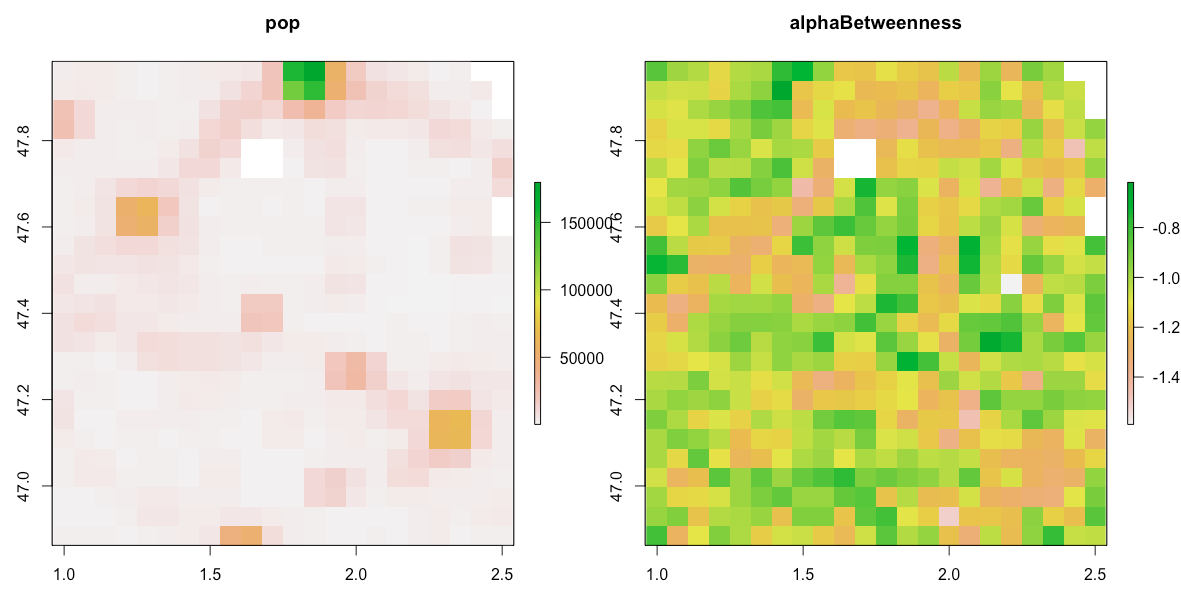
\includegraphics[width=\textwidth]{figures/pop-alphaBetweenness}





%%%%%%%%%%%%%%%%%%
\begin{figure}
\hspace{-5cm}
%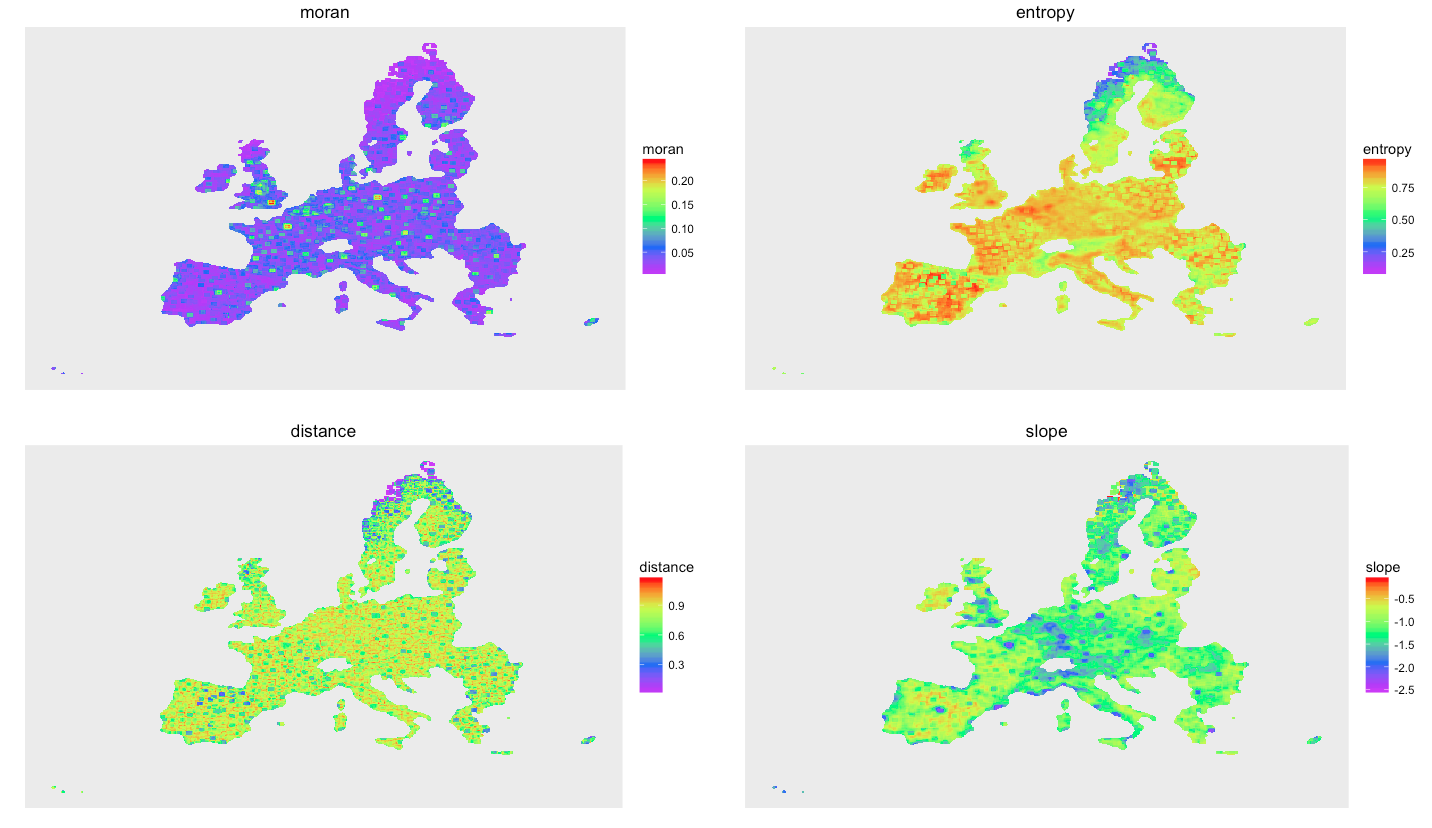
\includegraphics[angle=90,width=1.7\textwidth,height=\textheight]{Figures/Static/Density/all_50km}
\caption[Geographical Distribution of Morphologies][Distribution spatiale des indicateurs morphologiques]{Geographical Distribution of Morphologies : value of indicators across Europe.}{}
\end{figure}
%%%%%%%%%%%%%%%%%%


%%%%%%%%%%%%%%%%%%
\begin{figure}
\hspace{-3cm}
%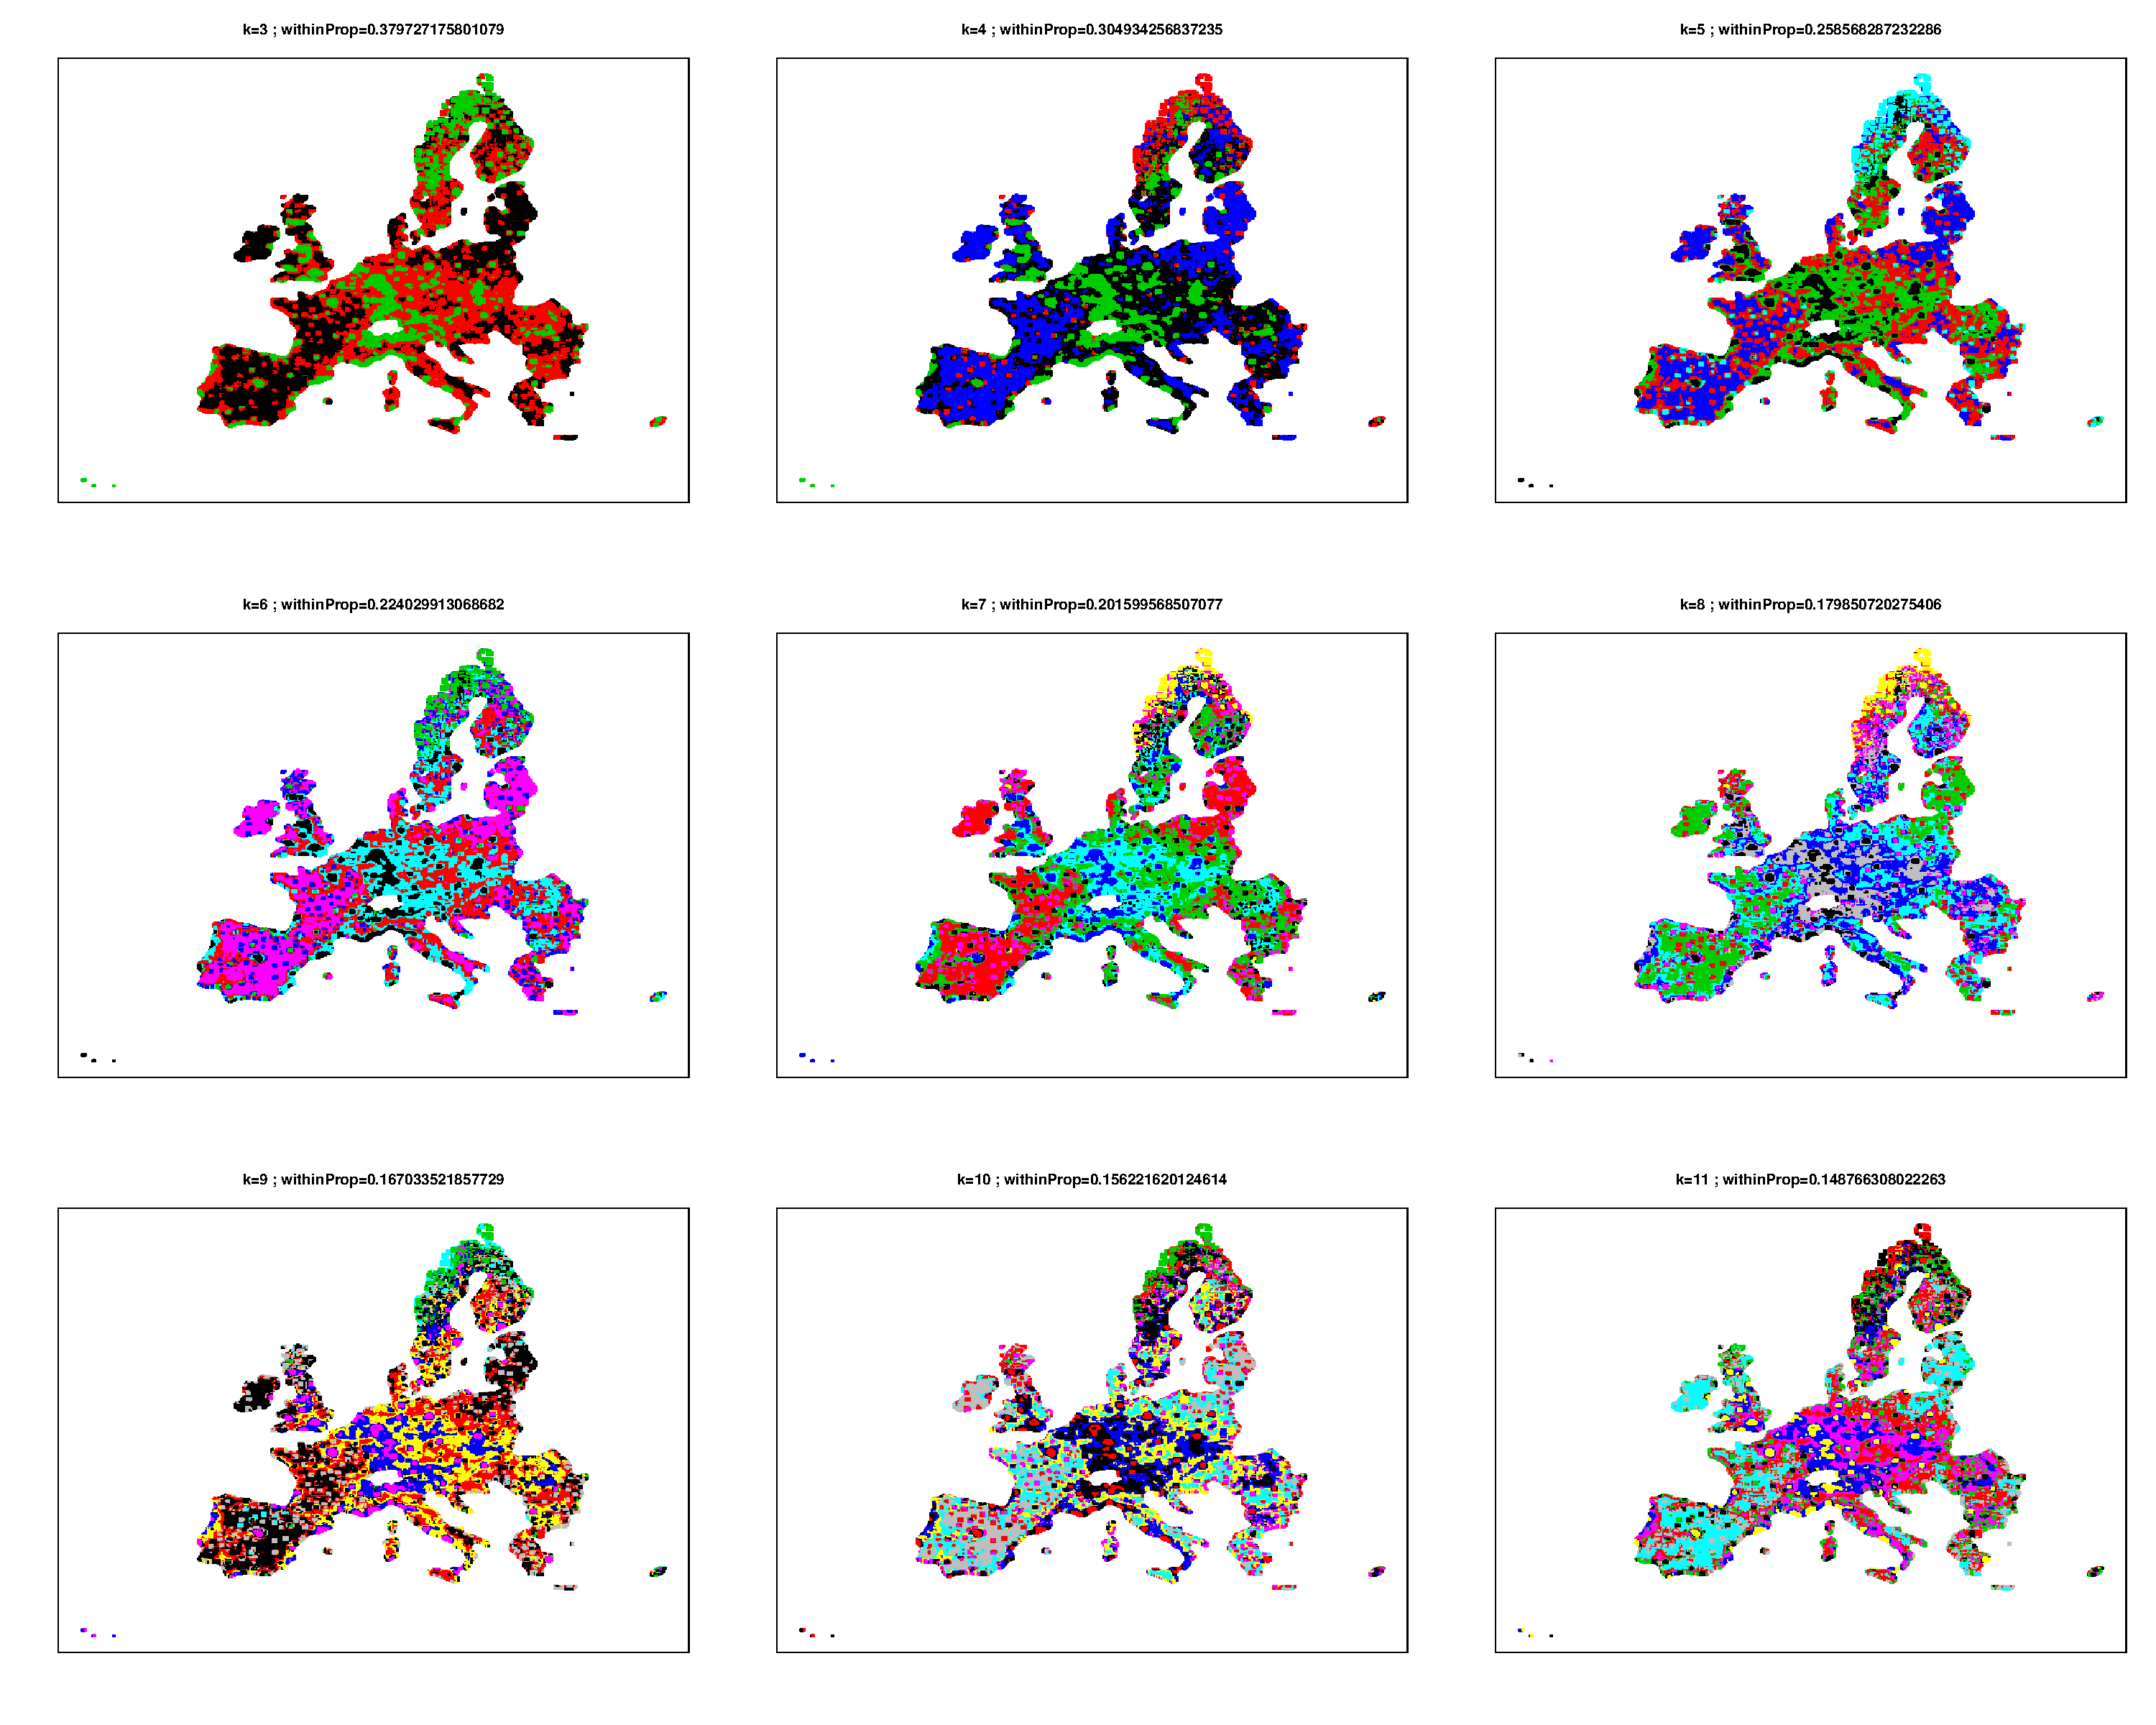
\includegraphics[angle=90,width=1.7\textwidth,height=\textheight]{Figures/Static/Density/clust_k3-11}
\caption[Clustering Analysis of Morphologies]{Clustering Analysis of Morphologies. We present the results of an average k-means for different values of }{}
\end{figure}
%%%%%%%%%%%%%%%%%%







%%%%%%%%%%%%%%%%%%
\subsection{Network Measures}{Mesures de Réseau}


\bpar{
We consider network aggregated indicators as a way to characterize transportation network properties on a given territory, the same way morphological indicators yielded information on urban structure. We propose to compute some simple indicators on same extents as for morphology, to be able to explore relations between these static measures. Static network analysis has been extensively documented in the literature, see for example \cite{louf2014typology} for a cross-sectional study of cities or \cite{2015arXiv151201268L} for exploration of new measures for the road network.
}{
Nous considérons les mesures agrégées de réseau comme un moyen de caractériser les propriétés des réseaux de transport sur un territoire donné, de la même façon que les indicateurs morphologiques informent sur la structure urbaine. Nous proposons de calculer des indicateurs simples sur des étendues spatiales similaires à la morphologie, pour être en mesure d'explorer les relations entre ces mesures statiques. L'analyse statique de réseau a été intensément documentée dans la littérature, voir par example \cite{louf2014typology} pour une étude comparative des villes ou \cite{2015arXiv151201268L} pour l'exploration de nouvelles mesures pour le réseau de rues.
}


\subsubsection{Data preprocessing}{Pré-traitement des données}


\bpar{
We work here with the road network, which structure is finely conditioned to territorial configuration of population densities. Furthermore, data for present day road network is openly available through the OpenStreetMap project~\cite{openstreetmap}. Its quality was investigated for different countries such as England~\cite{haklay2010good} and France~\cite{girres2010quality}. It was found to be of a quality equivalent to official surveys for the primary road network.
}{
Nous travaillons ici avec le réseau de rues, dont la structure est finement conditionnée aux configurations territoriales des densités de population. De plus, les données du réseau de routes actuel est disponible ouvertement par l'intermédiaire du projet OpenStreetMap (OSM)~\cite{openstreetmap}. Sa qualité a été étudiée pour différents pays comme l'Angleterre~\cite{haklay2010good} et la France~\cite{girres2010quality}. Il a été établi pour ces pays une qualité équivalente aux données officielles pour le réseau de rues primaire.
}


% data collected from http://download.geofabrik.de/europe.html

\bpar{
From the primary road segments, we compute the topological road network for all studied areas, at 100m granularity scale to be used consistently with the population grid. The OSM data is imported into \texttt{pgsql} using \texttt{osmosis}, is then aggregated at fixed granularity, and the resulting topological network is finally simplified with a split/merge algorithm.
}{
Pour les segments de rue primaires, nous calculons le réseau topologique pour l'ensemble des zones étudiées, à une granularité de 100m pour pouvoir être utilisé de manière cohérente avec les grilles de population. Les données OSM sont importées dans \texttt{pgsql} en utilisant \texttt{osmosis}~\cite{osmosis}, est ensuite agrégé à la granularité fixe, et le réseau topologique résultant est finalement simplifié avec un algorithme split/merge.
}

%
%\begin{columns}
%\begin{column}{width=0.7\textwidth}
%
%\end{column}
%\begin{column}{width=0.3\textwidth}
%\textit{.} % TODO summary stats here.
%\end{column}
%\end{columns}

%\begin{columns}
%\begin{column}{0.7\textwidth}
    %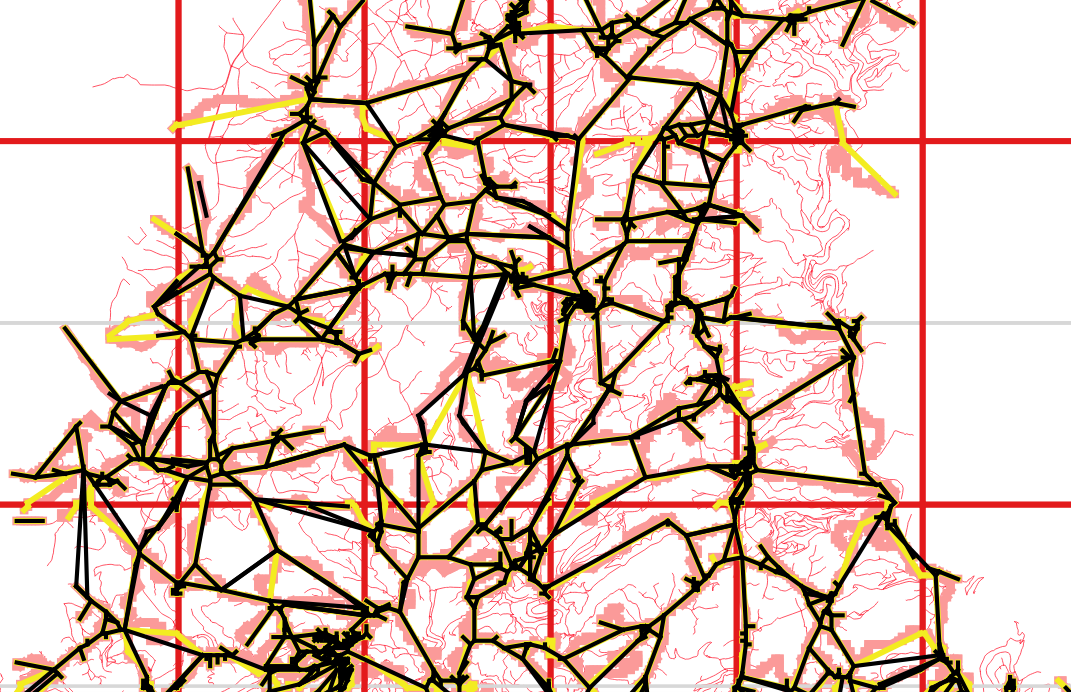
\includegraphics[width=\textwidth,height=0.5\textheight]{figures/ex_nw}
%\end{column}
%\begin{column}{0.3\textwidth}
   \textit{$\simeq 44\cdot 10^6$ links in initial OSM db, $\simeq 61\cdot 10^6$ in first simplified layer, $\simeq 21\cdot 10^6$ in final database}
%\end{column}
%\end{columns}






\paragraph{Simplification algorithm}{Algorithme de simplification}

For a given dataset corresponding to a subset of the overall road network, it is necessary to simplify network structure by spatial aggregation as initial data presents very detailed features and thus a very large numbers of nodes ($\simeq 10^10$ for Europe dataset). \comment{(Florent) c'est un peu confus, tu devrais d'abord dire : ce que tu as, les pb que ça pose, comment les résoudre}
 Such a level of precision is not needed in our study since density data is already aggregated at 500m resolution. It is possible to drastically reduce network size by spatial aggregation of nodes and link replacements. More precisely we use the following procedure :
\begin{itemize}
\item a background raster (which resolution $r$ gives the snapping parameter for aggregation) is constructed from a reference raster and the extent of network. This grid gives spatial aggregation units for network nodes.
\item for each feature of the road dataset, corresponding connected raster cells are stored with corresponding impedance and distance in a sparse adjacency matrix.
\item Network is simplified by iterative suppression of nodes with degree two, with keeping link speed and real length to their effective value.
\end{itemize}

% \cite{2016arXiv161101890B} : interactive appli for network simplification



\paragraph{Implementation}{Implémentation}

A \texttt{PostGIS} database is used to store raw and simplified network, in order to perform efficient spatial requests, compared for example to initial \texttt{osm} data formats (\texttt{osm} or \texttt{pbf}). However the size of storage of data into this base is much higher (factor 10) so processing was parallelized between european countries. Consistence is ensured by the use of the same common density raster as simplification canvas. Final network is stored into the Postgis database for efficient indicator computation given a spatial extent. \comment{(Florent) y'a t'il un effet de bord dans les carrés 50x50 qui se trouvent à la frontière de 2 pays}[pas avec nouvelle parallelisation pas par pays mais par split and merge (TODO rewrite nouvel algo)]


\paragraph{Sensitivity to simplification parameters}{Sensibilité aux paramètres de simplification}

Sensitivity of indicators to raster resolution and to degree simplification algorithm must still be tested to ensure the relevance of data preprocessing.


\subsubsection{Indicators}{Indicateurs}


\bpar{
Network macroscopic structure is summarized by the following set of indicators, after the simplifications and reductions done in the previous step. Assuming network given by $N=(V,E)$, nodes spatial positions $\vec{x}(V)$ and edges \emph{effective distances} $d(E)$ taking into account impedances and real distances (to include basically network hierarchy), we have indicators:
}{
Dans notre cas, nous résumons la structure macroscopique du réseau par un jeu fixé d'indicateurs, calculés sur les réseau topologiques obtenus par les étapes précédentes de simplification. Notant le réseau $N=(V,E)$, les noeuds ayant les positions spatiales $\vec{x}(V)$ et les liens des \emph{distances effectives} $d(E)$ qui prennent en compte les impédances et les distance réelle (pour inclure la hiérarchie primaire du réseau), nous avons les indicateurs :
}


\comment{(Florent) tb à présenter de la même manière, plus en même temps + justification pour la forme urbaine}


\todo{recompute indicators with capacity and/or hierarchy when possible with speed limits, to check how they change, and also correlations.}

\comment{(Florent) et entre les deux il y a donc les indicateurs d'accessibilité que tu as évacué trop vite je pense (d'autant qu'étant pile à l'interface forme urbaine/réseau - ils me semblent particulièrement indiqués vu ta problématique}




\begin{itemize}
\item connectivity
\item degree distribution
\item centrality, taken as normalized mean \emph{betweenness-centrality}
\item average path length
\item network diameter
\item mean network speed
\end{itemize}


L'accessibilité est bien considérée comme un indicateur de réseau, puisque son calcule implique d'attribuer des poids aux noeuds par un population correspondante.

\bpar{
These indicators are used to capture a rough picture of the structure. Refined work at smaller scales (intra-urban road network) and with more elaborated measures that allow to differentiate more precisely local form, was recently done by Lagesse in~\cite{2015arXiv151201268L}.
}{
Ces indicateurs sont utilisés pour avoir une idée large de la forme du réseau. Un travail plus élaboré à des échelles plus fines (réseau de rues intra-urbain) et avec des mesures plus raffinées permettant de discriminer localement des formes typiques, a été récemment mené par \noun{Lagesse} dans~\cite{2015arXiv151201268L}.
}



\subsubsection{Network Shape and Resilience}{Forme de Réseau et Résilience}

L'idée fondamentale motivant le calcul d'indicateurs de réseau est d'obtenir une réduction de dimension drastique, s'il est possible d'associer certains ``types'' de réseau à des valeurs typiques d'indicateurs. On est très loin d'une connaissance fine de typologies qui associeraient propriétés topologiques, dynamiques et processus de génération du réseau, le tout dans des typologies. De même que lier ces propriétés à des caractéristiques dérivées, comme la résilience qui est une propriété aux définitions diverses pour laquelle~\cite{Gao:2016ty} introduit une approche par la sensibilité des processus dynamiques. Afin d'illustrer d'une part la difficulté de caractériser les réseaux et d'autre part les potentialités offertes par notre base de données, nous développons en Appendice~\ref{app:sec:staticcorrelations} une courte analyse des propriétés de résilience au sens de~\cite{} pour des réseaux typiques.



\subsubsection{Results}{Résultats}


\bpar{}{
Les indicateurs de réseau ont été calculés sur les mêmes zones que les indicateurs de forme urbaine, 

}






%%%%%%%%%%%%%%%%%%
\subsection{Effective static correlations}{Correlations Statiques Effectives et Non-stationnarité}



%%%%%%%%%%%%%%%%%%
\subsubsection{Spatial Correlations}{Corrélations spatiales}




%%%%%%%%%%%%%%%%%
Results : Spatial Correlations

\textit{Computation of spatial correlation on square areas of width $\delta\cdot l_0$ (with typically $\delta = 4, \ldots , 16$)}


%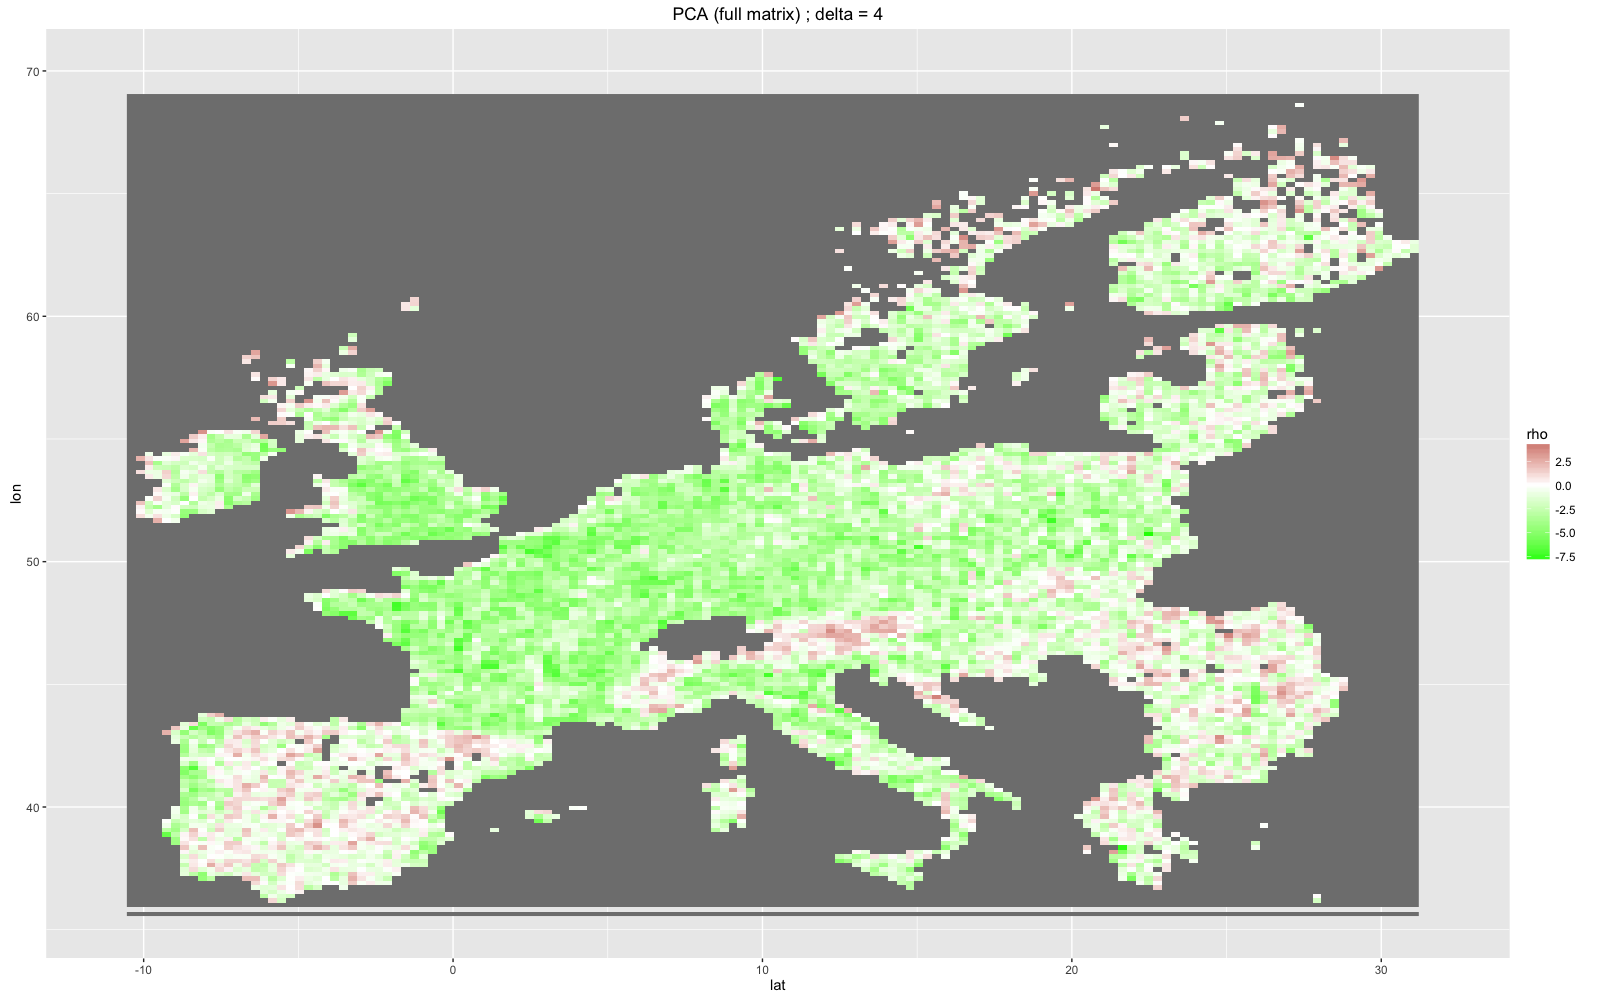
\includegraphics[width=\textwidth,height=0.7\textheight]{figures/corr_PCA_delta4}

$\rightarrow$ \textit{local spatial stationarity of processes}



%%%%%%%%%%%%%%%%%
%\sframe{Results : Stationarity scales}{
% maps
% 
%}



\paragraph{Multi-scale Processes}{Nature multi-scalaire des processus}

% plots
%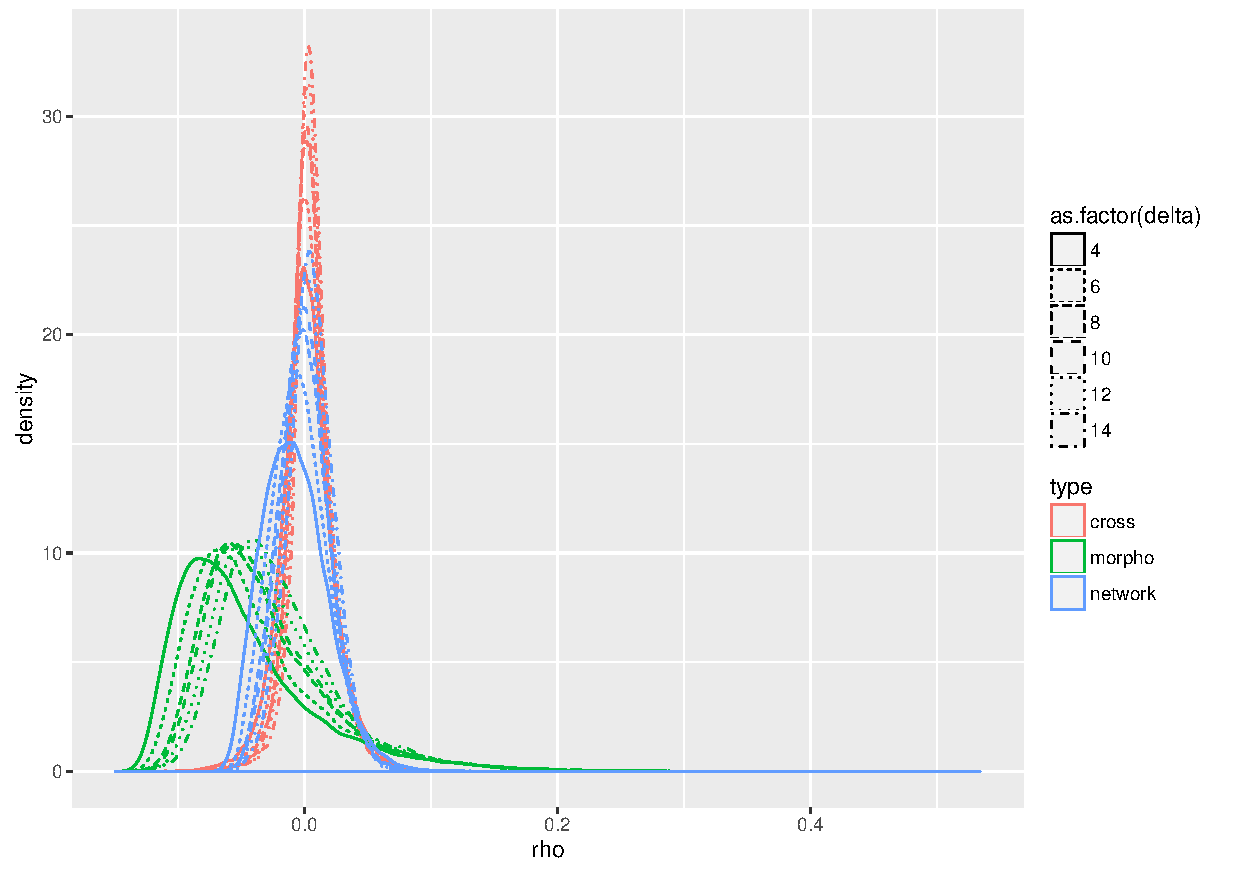
\includegraphics[width=0.33\textwidth]{figures/corrs-distrib_varyingdelta_bytype} % -> in supp material
%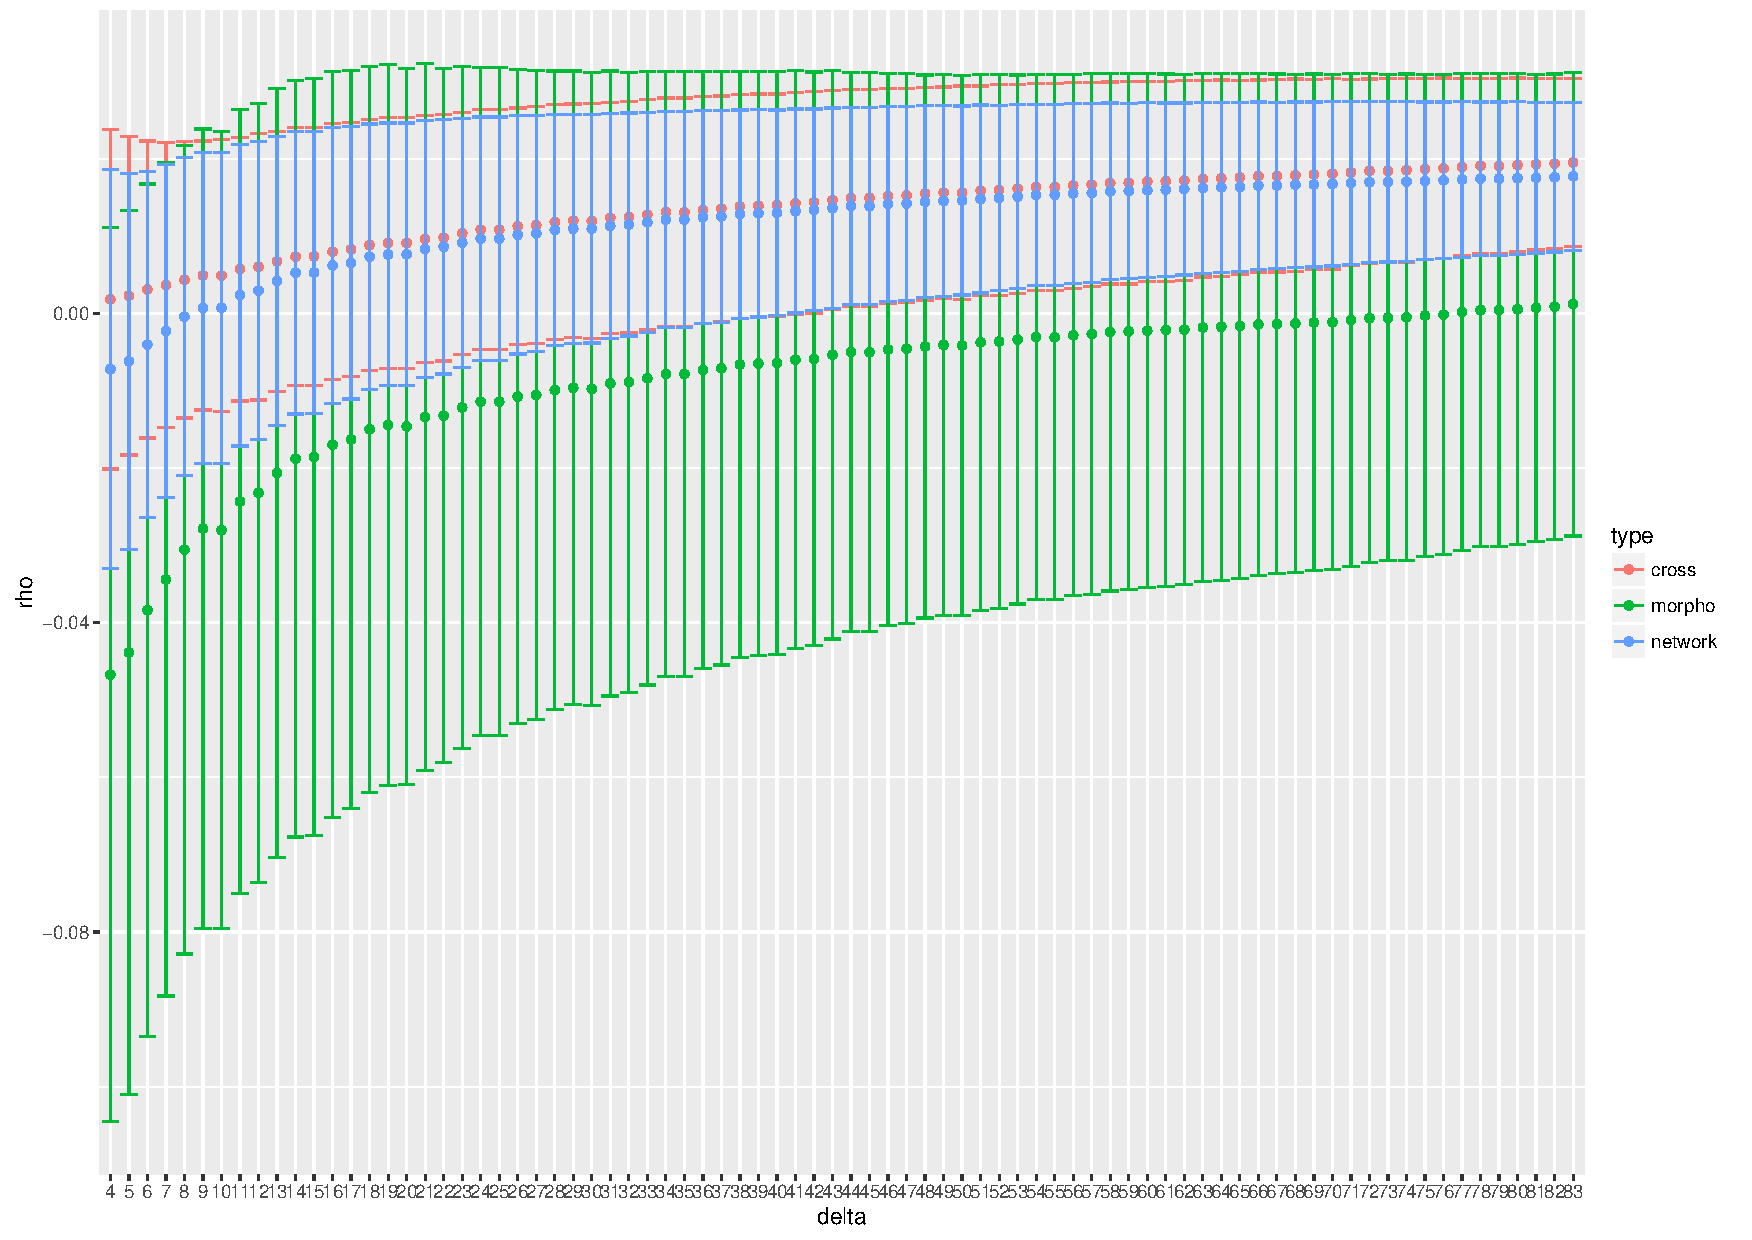
\includegraphics[width=0.5\textwidth]{figures/corrs-summary_varyingdelta_bytype_extended1}
%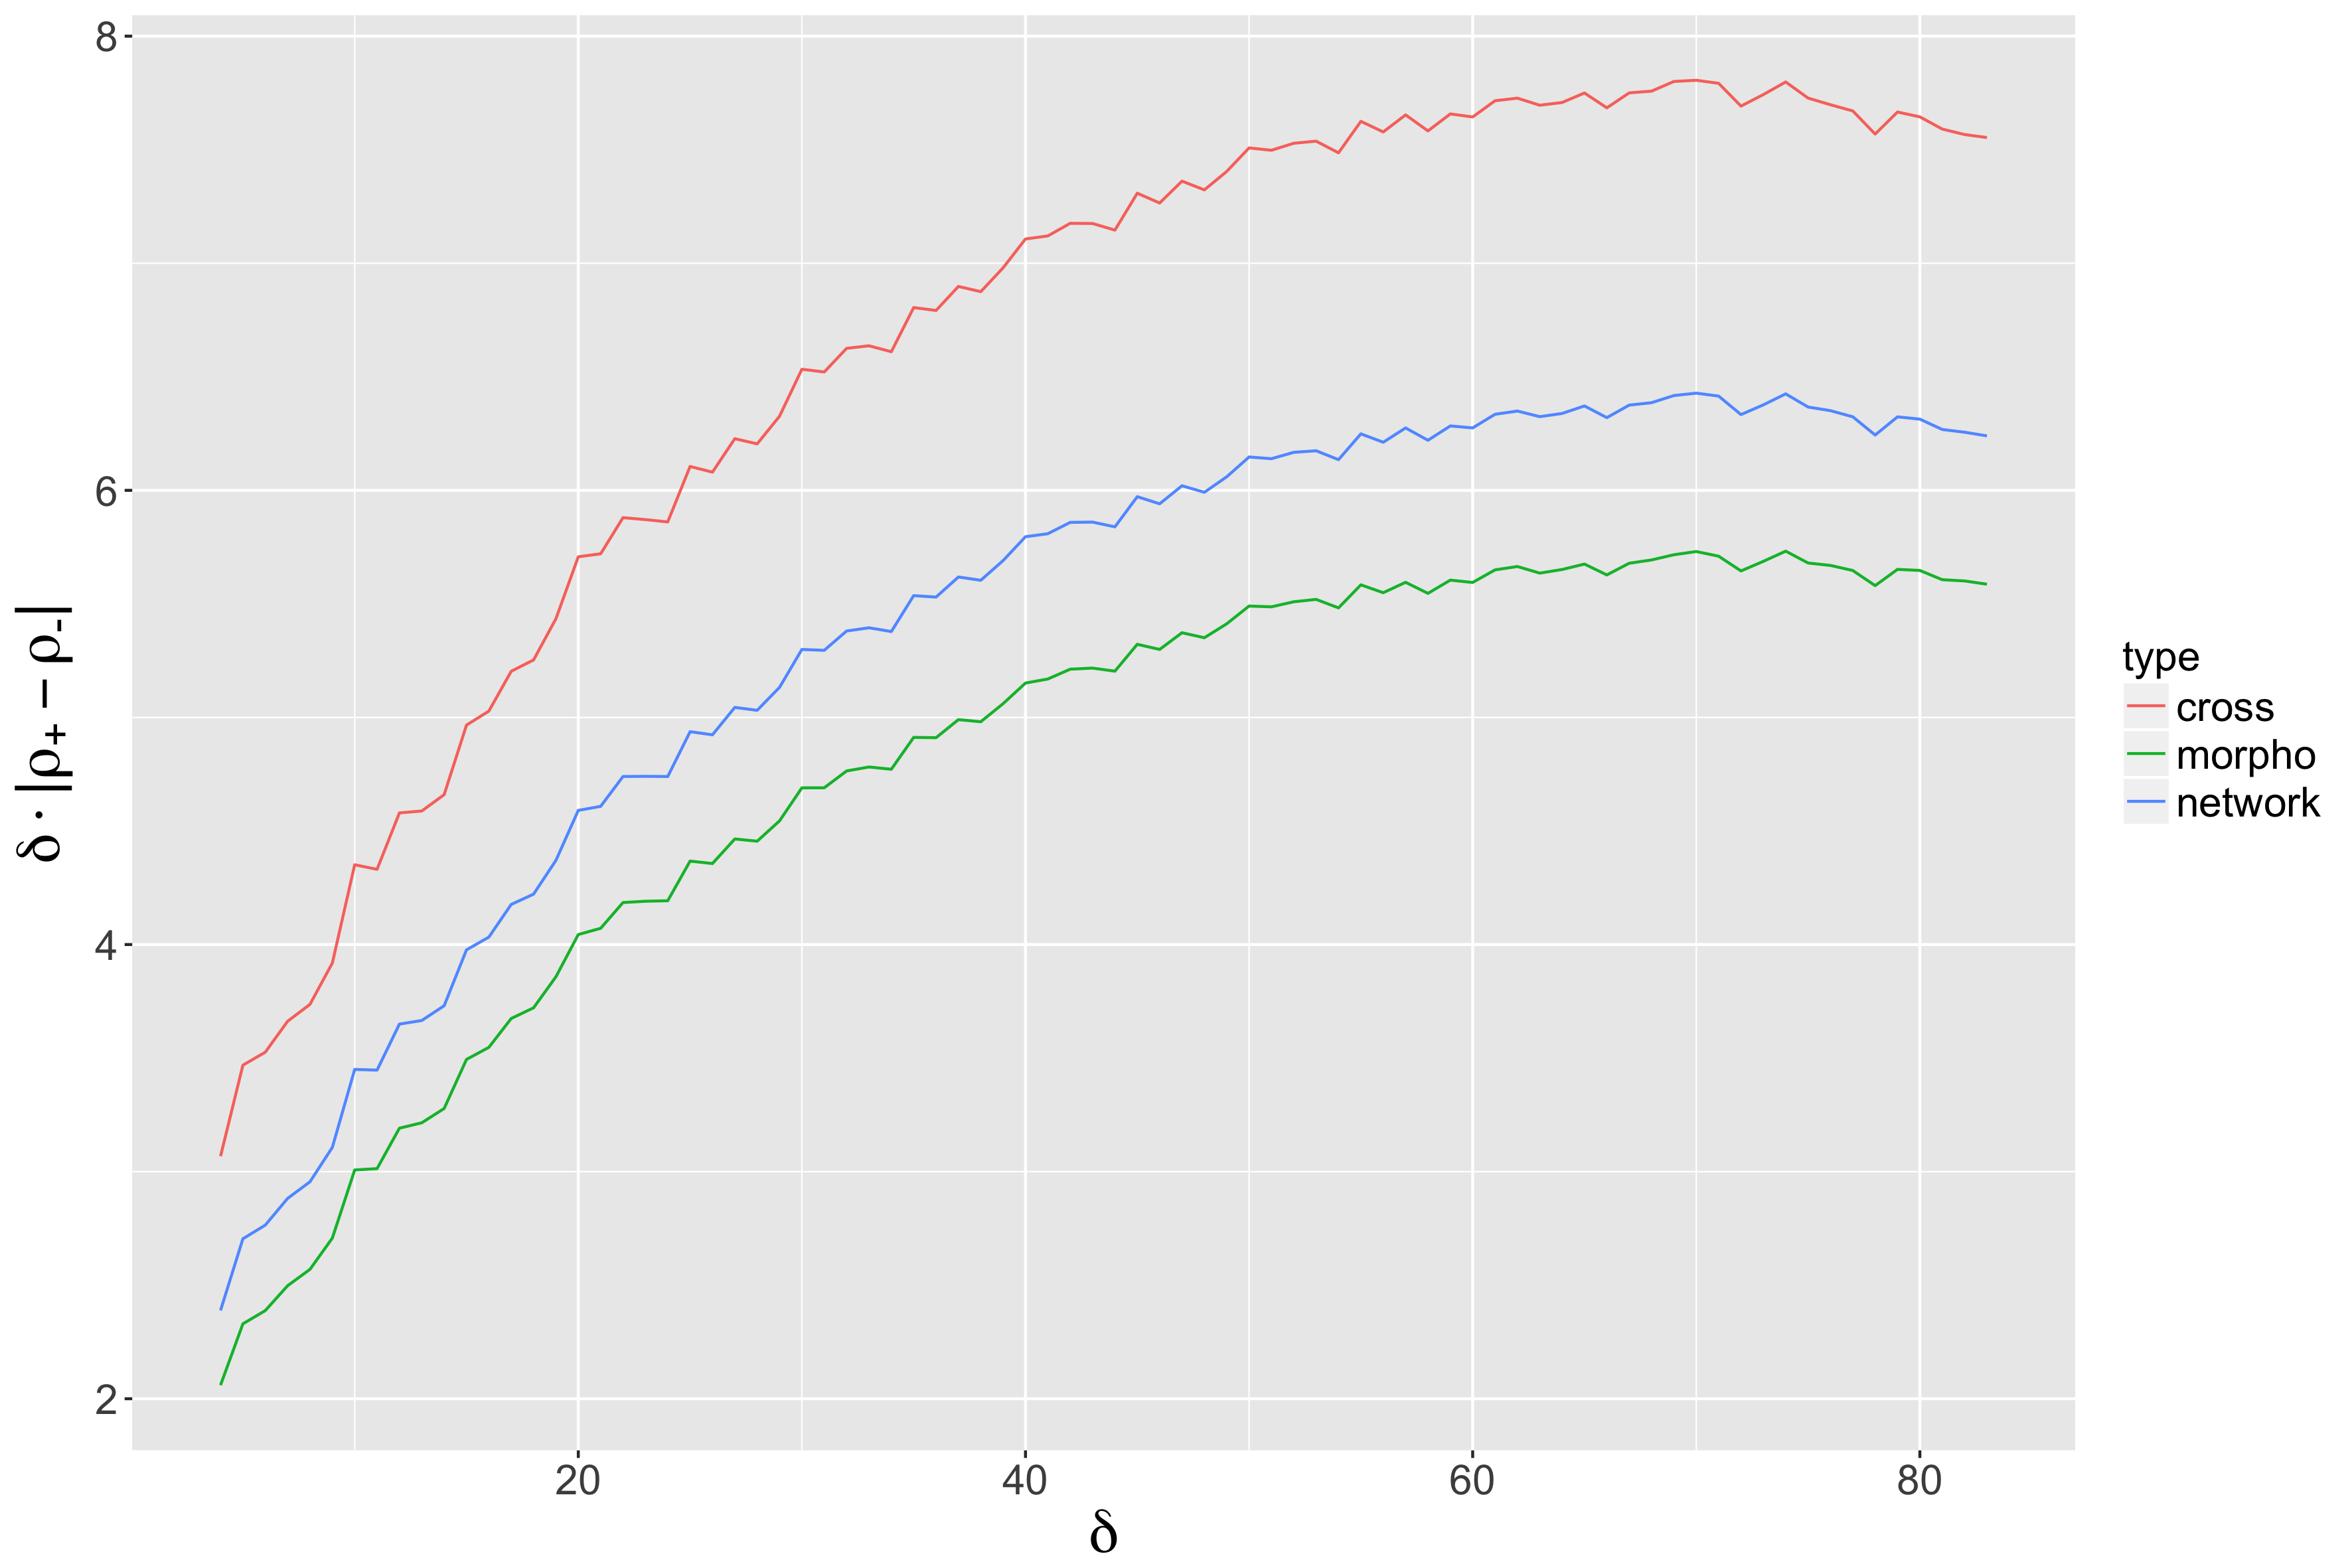
\includegraphics[width=0.5\textwidth]{figures/normalized_CI_delta}


On observe une variation significative des correlations moyennes en fonction de $\delta$

$\rightarrow$ Significant variation of mean correlation with $\delta$ (Left) and of normalized confidence interval (Right) given by $\left|\rho_+ - \rho_-\right|\cdot \delta$, as bounds theoretically vary as $\sqrt{N} \sim \sqrt{\delta^2}$ : implies multi-scalarity








%%%%%%%%%%%%%%%%%%
\subsubsection{Application to China}{Application à la Chine}


\bpar{
Although \cite{zheng2014assessing} underlined a quick acceleration of OpenStreetMap road data completeness and accuracy, its use for computation of network indicators may be questioned. \cite{zhang2015density} highlights four regimes of data quality, partitioning China into regions among which qualitative behavior of OSM data varies. We choose in the following to work only on the regions where the quality is the highest, i.e. with high density and high diversity. % TODO precise which areas
For density data, we use the gridded population data from~\cite{fu1km}. % TODO check also that
}{

}




In \cite{10.1371/journal.pone.0107042} density grids for other countries across the world (ex. China) are provided\footnote{available at \url{http://www.worldpop.org.uk/}} soo we may repeat our analysis to other regions for comparison purposes. \comment{(Florent) comparer quoi ?}









%%%%%%%%%%%%%%%%%%
\subsubsection{Spatial non-stationarity and non-ergodicity}{Non-stationnarité spatiale et non-ergodicité}
















Empirical Findings (Formalization)

$Y_i\left[\vec{x},t\right]$ spatio-temporal stochastic process, verifies empirically :

\bigskip

\begin{enumerate}
\item Local spatial autocorrelation is present and bounded by $l_{\rho}$ (in other words the processes are continuous in space) : at any $\vec{x}$ and $t$, $\left|\rho_{\norm{\Delta \vec{x}} < l_{\rho}}\left[Y_i (\vec{x}+\Delta \vec{x},t), Y_i (\vec{x},t) \right]\right| > 0$.
\medskip
\item Processes are locally parametrized : $Y_i = Y_i\left[\alpha_i\right]$, where $\alpha_i (\vec{x})$ varies with $l_{\alpha}$, with $l_{\alpha} \gg l_{\rho}$ and weakly locally stationary in space.
\medskip
%\item Spatial correlations between processes have a sense at an intermediate scale $l$ such that $l_{\alpha}\gg l \gg l_{\rho}$.
%\item Processes covariance stationarity times scale as $\sqrt{l}$.
%\item Local ergodicity is present at scale $l$ and dynamics are locally chaotic.
\item Processes are multi-scalar : since $\rho(\delta = \infty) > \rho (\delta = 0 )$, a necessary non-linear correction on processes spatial averages in correlation computation is present.
% add computation in supplementary materials / papers. -> later
\end{enumerate}



Analytical Deductions

1. \textbf{Regimes of temporal correlations.} Let assume local ergodicity in $\vec{x}_0$ at scale $\delta \cdot l_0$ (reasonable with urban growth and network extension in recent times). The Ergodic theorem implies that $\exists \mathcal{T}$ such that

\[<Y_i (t) >_{\norm{\vec{x}-\vec{x}_0} < \delta\cdot l_0} = <Y_i (\vec{x}_0)>_{t\in \mathcal{T}}\] 

With spatial stationarity, $<Y_i>_{\vec{x}_0}=<Y_i>_{\vec{x}_1}$, thus $\mathcal{T}$ must be constant to be invariant by translation. By contraposition and (2), processes have different dynamical characteristics.
% if translate in a given direction, looses a small part, must be compensated by the area translated by delta (overlap), thus must be constant.

\bigskip

2. \textbf{Global non-ergodicity.} Let $X_k$ a partition of space into local areas. We have $<\cdot>_x = \sum_k w_k <\cdot>_{x_k} =_{(1)} \sum_k w_k <\cdot>_{\mathcal{T}_k} $. On the other hand, global ergodicity would give $<\cdot>_t = <\cdot>_{\mathcal{T}} = \sum_k w_k <\cdot>_{\mathcal{T}}$ and $\sum_k w_k \left(<\cdot>_{\mathcal{T}} - <\cdot>_{\mathcal{T}_k}\right) = 0$. Being true on each subset implies $\mathcal{T}=\mathcal{T}_k$, what contradicts (1).





%
%
%%%%%%%%%%%%%%%%%%
%\sframe{Stationarity and Ergodicity}{
%
%\begin{itemize}
%\item Assuming local ergodicity, spatial local stationarity implies and temporal local stationarity
%
%\item Spatial non-stationarity \textbf{at the second order}$\implies$ temporal scale variations $\implies$ non-ergodicity
%
%\end{itemize}
%
%}
%




Case study : implications
% thematic conclusion of the case study on ergodicity

$\rightarrow$ Still points to explore :
\begin{itemize}
\item variable correlations areas (size and shape in space)
\item same work on cities population/train network data, which are also dynamical databases : extrapolation of ergodicity parameters ?
\item correlations of returns : link between $\rho\left[\Delta_t Y\right]$ and $\rho\left[\Delta_x Y\right]$ (more difficult : if pure local ergodicity, $\exists$ a permutation making the correspondance) % may be difficult to identify 
\item Link between $\Delta_{\delta}\rho (\delta)$ and process derivatives ?
\end{itemize}

\bigskip

$\rightarrow$ We show the regional nature of network-territories interactions, in particular the non-ergodicity of urban systems on \textbf{the interaction these components}

\bigskip

$\rightarrow$ No direct results on time dynamics, but indirect : spatio-temporal processes do not have same speed and react/diffuse differently
















